\documentclass{bredelebeamer}

%%%%%%%%%%%%%%%%%%%%%%%%%%%%%%%%%%%%%%%%%%%%%%%%

\title[Gana++ Sprint 3]{Gana++ Sprint 3}
% Titre du diaporama

\subtitle{Proceso de migración de datos a MongoDB}
% Sous-titre optionnel

\author{Gana+ Back-End}%\inst{1}
% La commande \inst{...} Permet d'afficher l' affiliation de l'intervenant.
% Si il y a plusieurs intervenants: Marcel Dupont\inst{1}, Roger Durand\inst{2}
% Il suffit alors d'ajouter un autre institut sur le modèle ci-dessous.

\institute[Hundred]
{
 % \inst{1}
  Elmer Cangahuala\\
  César Cárdenas\\  
  Alexander \\
  Juan Lucero\\
  }


\date{30 de Agosto 2018}
% Optionnel. La date, généralement celle du jour de la conférence

\subject{Sujet de votre diaporama}
% C'est utilisé dans les métadonnes du PDF

\logo{

\includegraphics[scale=0.15]{imgs/logoHundred.png}
}


%%%%%%%%%%%%%%%%%%%%%%%%%%%%%%%%%%%%%%%%%%%%%%%%%%%%%%%%%%
%%%%%%%%%%%%%%%%% 			INICIO			%%%%%%%%%%%%%%%%%%%%%%%
%%%%%%%%%%%%%%%%%%%%%%%%%%%%%%%%%%%%%%%%%%%%%%%%%%%%%%%%%%
\begin{document}

\begin{frame}
  \titlepage
\end{frame}

\begin{frame}{Contenido}
  \tableofcontents
  % possibilité d'ajouter l'option [pausesections]
\end{frame}

%%%%%%%%%%%%%%%%%%%%%%%%%%%%%%%%%%%%%%%%%%%%%%%%%%%%%%%%%%
%%%%%%%%%%%%%%%%% 			SECCION 1			%%%%%%%%%%%%%%%%%%%%%%%
%%%%%%%%%%%%%%%%%%%%%%%%%%%%%%%%%%%%%%%%%%%%%%%%%%%%%%%%%%
\section{Proceso de carga inicial}
\begin{frame}{Proceso de carga inicial}
\begin{figure}
\centering
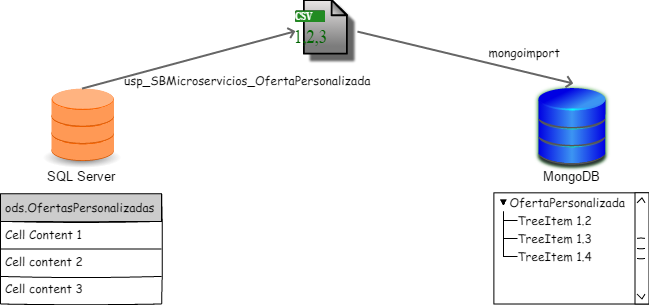
\includegraphics[scale=0.35]{imgs/OfertaPersonalizada.png}
\end{figure}
\end{frame}

\subsection{Migración de ofertas personalizadas}
\begin{frame}{Migración de ofertas personalizadas}
\begin{figure}
\centering
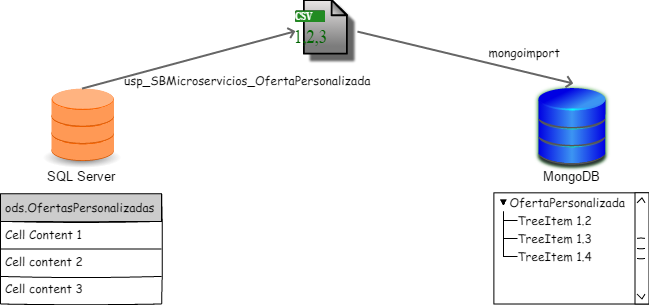
\includegraphics[scale=0.35]{imgs/OfertaPersonalizada.png}
\caption{OfertaPersonalizada.cmd}
\end{figure}
\end{frame}

\begin{frame}{Migración de ofertas personalizadas CUV}
\begin{figure}
\centering
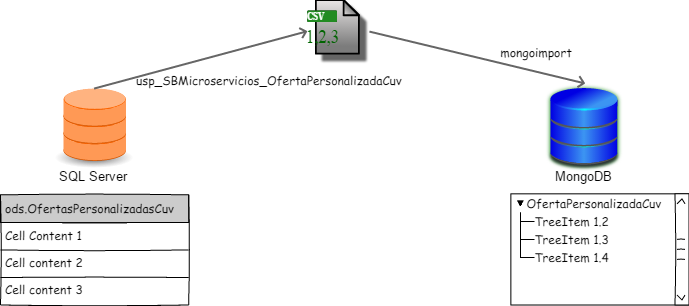
\includegraphics[scale=0.35]{imgs/OfertaPersonalizadaCuv.png}
\caption{OfertaPersonalizadaCuv.cmd}
\end{figure}
\end{frame}

\subsection{Migración de tipo estrategia}
\begin{frame}{Migración de tipo estrategia}
\begin{figure}
\centering
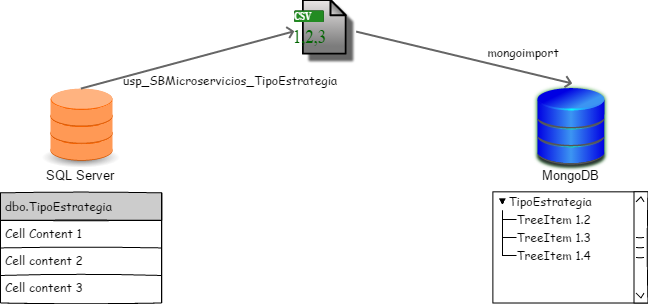
\includegraphics[scale=0.35]{imgs/TipoEstrategia.png}
\caption{TipoEstrategia.cmd}
\end{figure}
\end{frame}

\subsection{Migración de producto comercial}
\begin{frame}{Migración de producto comercial}
\begin{figure}
\centering
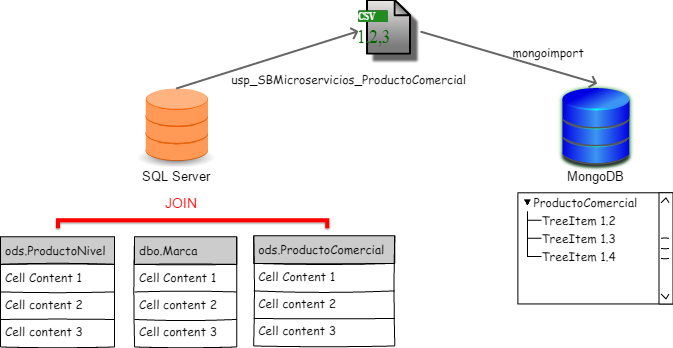
\includegraphics[scale=0.35]{imgs/ProductoComercial.png}
\caption{ProductoComercial.cmd}
\end{figure}
\end{frame}

\subsection{Migración de producto faltante}
\begin{frame}{Migración de producto faltante}
\begin{figure}
\centering
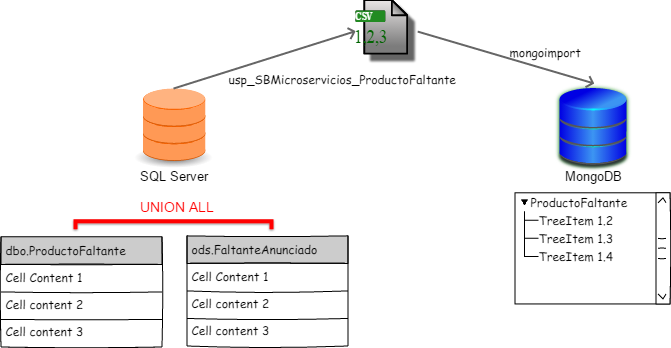
\includegraphics[scale=0.35]{imgs/ProductoFaltante.png}
\caption{ProductoFaltante.cmd}
\end{figure}
\end{frame}

\subsection{Migración de tonos}
\begin{frame}{Migración de tonos}
\begin{figure}
\centering
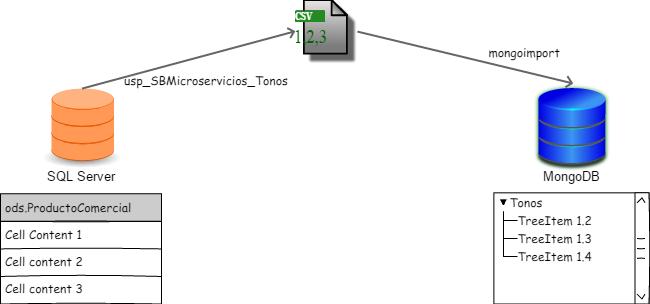
\includegraphics[scale=0.35]{imgs/Tonos.png}
\caption{Tono.cmd}
\end{figure}
\end{frame}

\subsection{Migración de Estrategias}
\begin{frame}{Migración de Estrategias}
\begin{figure}
\centering
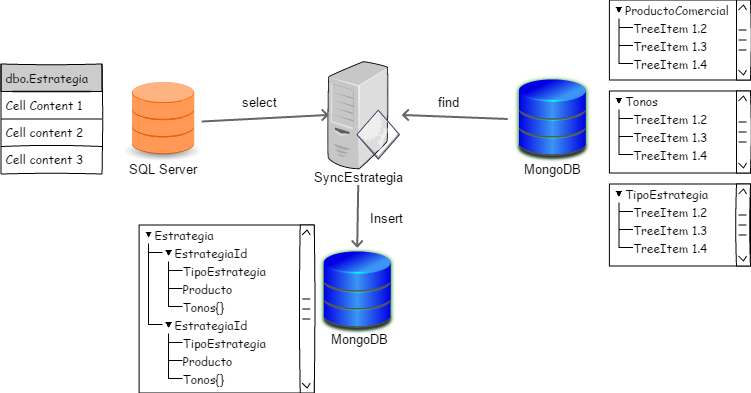
\includegraphics[scale=0.35]{imgs/Estrategia.png}
\caption{InitEstrategiasAll()}
\end{figure}
\end{frame}

%%%%%%%%%%%%%%%%%%%%%%%%%%%%%%%%%%%%%%%%%%%%%%%%%%%%%%%%%%
%%%%%%%%%%%%%%%%% 			SECCION 2			%%%%%%%%%%%%%%%%%%%%%%%
%%%%%%%%%%%%%%%%%%%%%%%%%%%%%%%%%%%%%%%%%%%%%%%%%%%%%%%%%%
\section{Proceso de sincronización}
\begin{frame}{Proceso de sincronización}
\end{frame}

\subsection{Sincronización de Estrategias}
\begin{frame}{Sincronización de Estrategias}
\begin{figure}
\centering
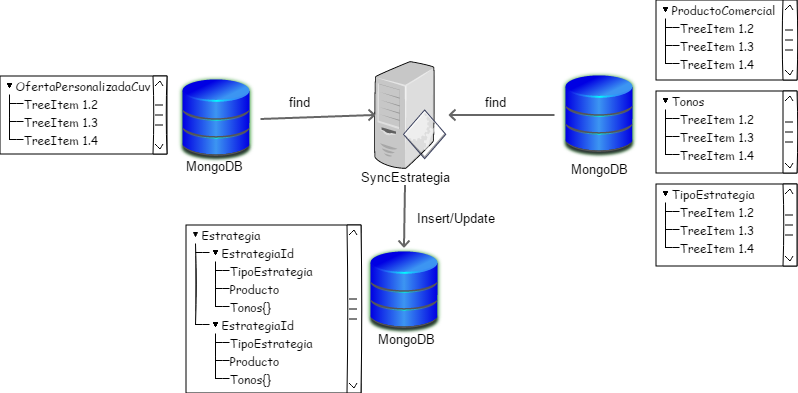
\includegraphics[scale=0.35]{imgs/EstrategiaLoad.png}
\caption{LoadEstrategiasAll()}
\end{figure}
\end{frame}

\end{document}